\section{\label{sct:modules}Modules}

A complete Amber system will comprise at least three modules running at the
same time; there is a Crawler module, a selector module called Sieve and a
display called ShowOff. The modules are separate executables with their own
life-cycles and resources.

Every module has a specified interface through which communication with
Psyclone is handled.

\subsection{Crawler modules}

\begin{figure}
    \centering
    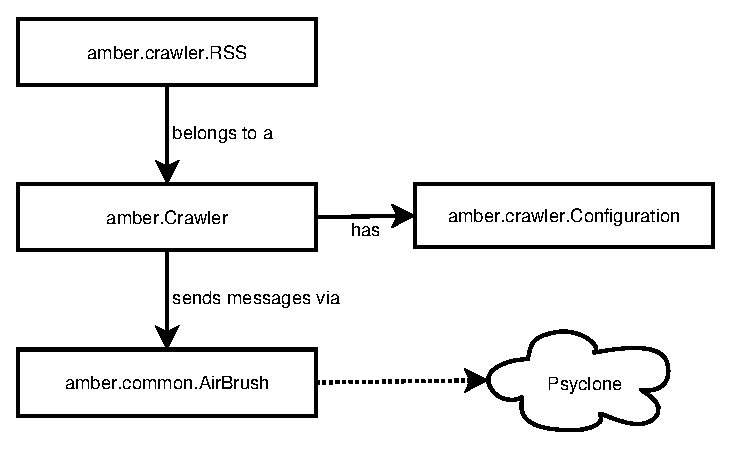
\includegraphics{image/crawler}
    \caption{Diagram of the design of the Crawler, the names are Java classnames}
\end{figure}

When the Crawler is started, it will create one of the available handlers
(depending on what is specified on the command line or what is set as default
during build time). 

It also creates an AirBrush instance to communicate with Psyclone via
Java\-Open\-AIR. The module name announced to Psyclone is `Crawler.' plus the
name of the handler, so `Crawler.RSS' in case of the RSS handler.

After connecting with Psyclone, the handler can get its parameters stored in
the psySpec file and go to work. It will post stories with type
`External.Crawler.$\langle$handler$\rangle$.Story' (i.e.
`External.Crawler.RSS.Story') on the whiteboard `WB.Stories.Raw'.

\subsubsection{RSS}

The RSS crawler module will be fairly straightforward. There are actually quite
a few good RSS parsers around for Java, the only thing the crawler should do is
getting the stories from the RSS feeds along with meta-information and store it
on the whiteboard.

\begin{module}{Crawler.RSS}
    \post{External.Crawler.RSS.Story}{WB.Stories.Raw}
\end{module}

\subsubsection{DiggAPI}

Digg is a website which lets users submit stories found on the web. Other users
then moderate the submissions either by `digging' or `burying' a story. A story
with a lot of `diggs' is a popular one. The nice thing about Digg is that it
actually does a lot of work for the \Amber\ system.

Digg
announced\footnote{\url{http://diggtheblog.blogspot.com/2006/07/digg-labs-launches-alpha.html}}
that they will publish a public API within the next months. If time allows, a
DiggAPI module is created.

\begin{module}{Crawler.DiggAPI}
    \post{External.Crawler.DiggAPI.Story}{WB.Stories.Raw}
\end{module}

% \subsubsection{BloggerDataAPI}
% 
% One of the larger weblog hosters is Google with their Blogger service. There
% is an API available to get information from it.

\subsection{Sieve modules}

Every invocation of a Sieve on a Story will decrease its \texttt{processLeft}
value until it is 0. When it reaches 0, the story is moved to the ``processed''
whiteboard WB.Stories.Processed.

\subsubsection{KeywordSpotter}

The KeywordSpotter is configured to detect the presence of certain keywords in
a story which makes it fit in a certain category or subject. In early versions
the weights of the subjects will be equal. In later versions all weights of all
subjects of a story must for instance add up to 100\%. This gives the
visualizer more freedom to place the story.

\begin{module}{Sieve.KeywordSpotter}
    \post{Internal.Story}{WB.Stories.Processed}
    \post{External.Crawler.*.Story}{WB.Stories.Raw}
    \trigger{External.Crawler.*.Story}{WB.Stories.Raw}
\end{module}

\subsubsection{PhraseSpotter}

The PhraseSpotter will use a grammar engine to detect whether certain types of
sentences appear in a story to classify it.

% \begin{module}{Sieve.PhraseSpotter}
% \end{module}

\subsection{ShowOff modules}

\begin{figure}
    \centering
    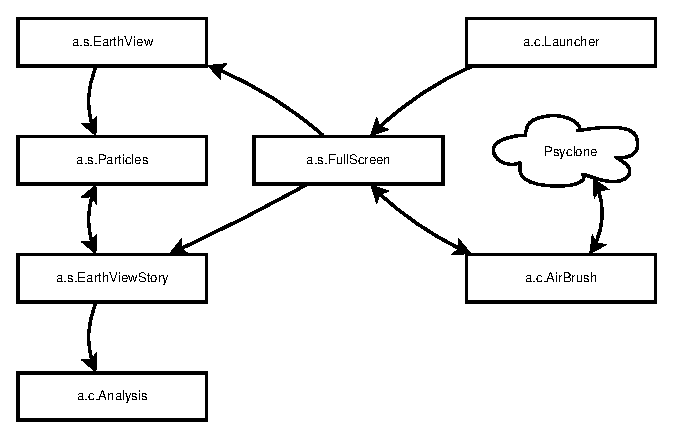
\includegraphics{image/showoff-fullscreen}
    \caption{Diagram of the design of the full screen ShowOff module, the names are abbreviated Java classnames}
\end{figure}

\subsubsection{Full screen}

The full screen application will display a lot of information and is there to
be looked - not glanced - at. It should be possible to let it do its job
autonomously, just showing a pretty picture, or to be interactive.

\begin{module}{ShowOff.FullScreen}
    \trigger{Internal.Story}{WB.Stories.Processed}
\end{module}

\subsubsection{Ambient applet}

The ambient applet will display a very easy to understand image of the status
of the page it is on. I.e. if the page is a weblog, it should display subject
information on that weblog, if it is on the page of a thread of a forum, it
displays the flow of the discussion.

\begin{module}{ShowOff.Applet}
    \trigger{Internal.Story}{WB.Stories.Processed}
\end{module}

